\clearpage
\section{Material and methods}\label{sec:ukb-methodology}
%%%%%

In this section we describe how we \emph{analyze} the data and cohorts and described in the previous section.
We apply techniques and frameworks discussed in the previous chapters.

%%
\subsection{TVFC estimation method}
%%

Based on our benchmarking work in the previous chapter, how should we now estimate \gls{tvfc}?
The goal of the benchmarking framework was to pick the best method available.
Based on \cref{ch:benchmarking}, at the time of writing the evidence points toward the \gls{wp} approach for being the best overall \gls{tvfc} estimation method.
However, if new methods are developed that outperform the \gls{wp} model on these benchmarks, or if additional benchmarks paint a different picture, the experiments in this current chapter should be re-run and conclusions updated accordingly.
More specifically, we pick \gls{svwp} for computational efficiency, as $N > 400$.

Alternatively (or perhaps complementary), as argued in \cref{subsec:benchmarking-reflection}, we can use our imputation benchmark on the actual data of interest to pick the optimal \gls{tvfc} estimation method.
We only run this benchmark on the individual brain \glspl{roi} data ($D = 9$), not the \gls{fn} node time series.
Moreover, we run it once on all broadly eligible participants, instead of separately for each cohort stratification.
%
The results are shown in \cref{fig:ukb-imputation-benchmark}.
We see the pairwise implementation of \gls{dcc} performing similarly to the joint implementation, suggesting limited edge-specific dynamics.
However, neither \gls{dcc} implementation outperforms the \gls{sfc} estimates.
Furthermore, we see both the \gls{svwp} and \gls{sw-cv} approaches outperform the static estimate.
This is interpreted as (at least) some edges having a non-stationary covariance structure.
Overall, the \gls{svwp} approach performs best, solidifying our decision to use it for estimating \gls{tvfc} in this study.


\begin{figure}[ht]
  \centering
  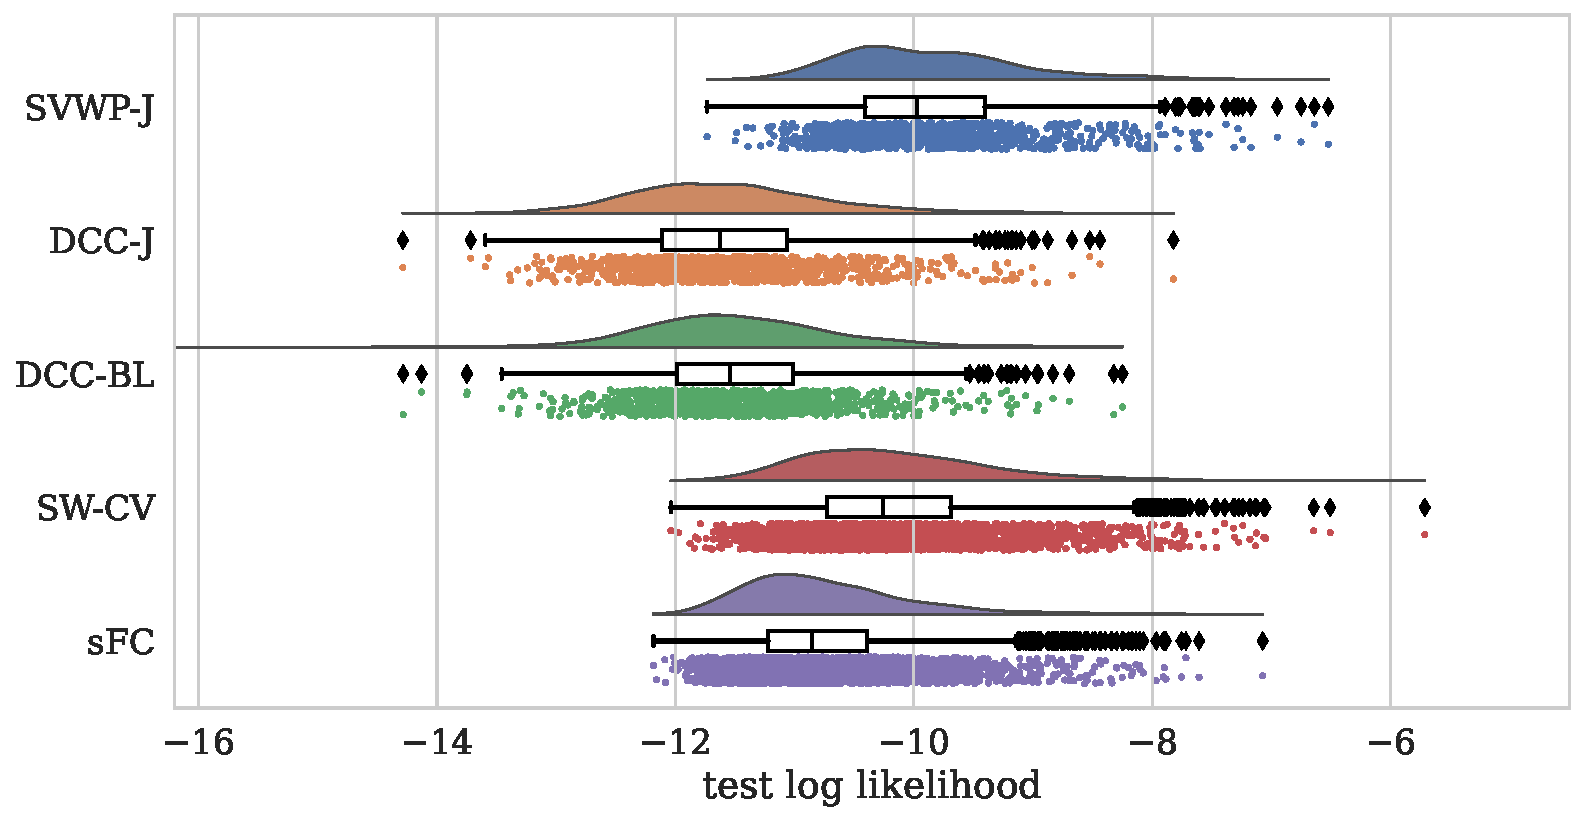
\includegraphics[width=\textwidth]{fig/ukbiobank/imputation_study/ROI/LEOO_test_log_likelihoods_raincloud}
  \caption{
    UK Biobank depression study imputation benchmark test log likelihoods.
    The SVWP approach performs best.
  }\label{fig:ukb-imputation-benchmark}
\end{figure}


We also run all experiments and analyses with the other \gls{tvfc} estimation methods discussed previously.
This will illustrate if and how scientific conclusions are impacted by the (seemingly arbitrary) researcher choice of \gls{tvfc} estimation method (see Appendix~\ref{appendix:more-ukb-results} for these results).
These methods are \gls{dcc} (both trained jointly and as bivariate loop) and \gls{sw-cv}.
Furthermore, we run the analyses with a simple \gls{sw} with window length of both 30 and 60 seconds, mimicking what could be considered a standard analysis procedure.
Lastly, all analyses are compared to the \gls{sfc} analysis (where applicable).

%%
\subsection{Cohort comparison}
%%

We compare cohorts in a straightforward manner by computing and comparing \gls{tvfc} estimate summary measures for the brain region edges of interest subset and all three \gls{fn} interactions.

To assess the significance of contrasts between cohorts, we apply methods from the Neyman-Pearson (i.e.~standard, orthodox) school of statistical hypothesis testing.\footnote{See \textcite{Dienes2008} for an excellent and complete overview of the various schools of thought.}
%
We run two-sample $t$-tests on the \gls{tvfc} summary measures across all subjects for the edges of interest.
To correct for multiple comparisons, we run both the Bonferroni (which is often considered too conservative) as well as the Benjamini-Hochberg \gls{fdr} method~\parencite{Benjamini1995}, using $\alpha = 0.05$ as significance threshold (as is traditional).
All figures show significance indications after the latter correction.
These \gls{mht} corrections are considered separately for each \gls{tvfc} summary measure, as they are considered independent from one another.
%
As we anticipate small effect sizes (see \cref{subsec:fc-depression}), we report Cohen's $d$ where appropriate~\parencite{Cohen1988, Lakens2013}.
To get a ball-park interpretation of effect size, \textcite{Cohen1988} suggested `small' ($d = 0.2$), `medium' ($d = 0.5$), and `large' ($d = 0.8$) as effect size labels.
However, he already noted that these are rather arbitrary and should only be used if findings are so novel that they cannot be compared to prior findings.
Relating effect sizes to previous findings is indeed its most useful application.
Unfortunately, not everyone reports these.

%%
\subsection{Brain state analysis}
%%

We also investigate cohort \gls{tvfc} characteristics and contrasts through the construct of brain states (see \cref{subsec:brain-states} for explicit definition).
These are extracted separately for each of the four analysis types (i.e.~cohort stratifications).
All nine \glspl{roi} are included.
%
We extract $k = 4$ brain states, based on the elbow plot as shown in \cref{fig:ukb-results-brain-states-elbow-plot}.
However, the absence of a clear `elbow point' may indicate that there is not as much of a distinct cluster data structure.


\begin{figure}[t]
  \centering
  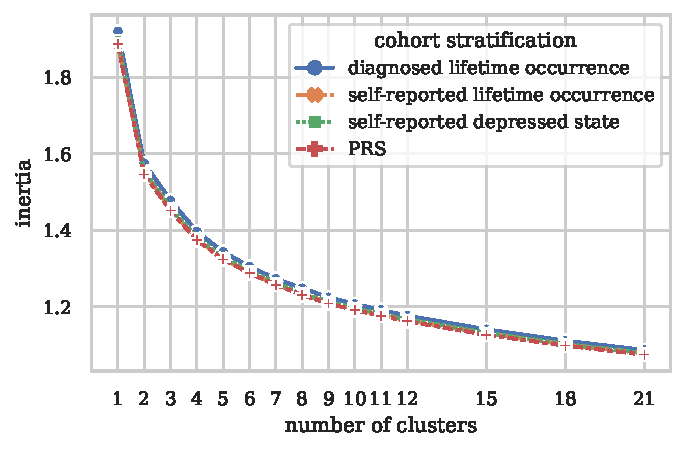
\includegraphics[width=0.8\textwidth]{fig/ukbiobank/brain_states/inertias_SVWP_joint}
  \caption{
    UK Biobank brain state analysis inertia elbow plot - SVWP-J estimates.
    Used for determining optimal number of clusters.
    Lines overlap heavily for all four cohort stratifications.
  }\label{fig:ukb-results-brain-states-elbow-plot}
\end{figure}


%%
\subsection{Predictive power as explanation}
%%

One key insight from the benchmarking efforts is that it not only allows us to pick the optimal \gls{tvfc} estimation method.
It also paints a broader picture and a profile of predictive power.
Such maps between edge connectivity and predictive power of subject measures, for example, can be useful when interpreting results.
This is especially relevant in an interdisciplinary field like this.
This is exactly the philosophy that led to the recent publication of the open-source Python package \texttt{neuromaps}~\parencite{Markello2022}.

This mindset constitutes a very pure data science view of the brain and neuroscience as a field~\parencite[see also][]{Yarkoni2017}.
Machine learning as a field has fully embraced this mindset.\footnote{The fields of \gls{nlp} and acoustic modeling have slowly shifted away from mechanistic language models to purely statistical approaches. In 1988, speech recognition pioneer Frederick Jelinek famously said something along the lines of ``Every time I fire a linguist, the performance of the speech recognizer goes up'' (exact wording is lost in time).}
It may not be a silver bullet, and does not necessarily lead to mechanistic understanding and strong theory~\parencite[see e.g.][]{Jonas2017}.
However, it is certainly a promising research direction that may help bridge brain dynamics and brain function, a key bottleneck often raised in the field~\parencite{Kopell2014}.
Moreover, some psychiatrists have called for prioritizing predictive power and clinical utility in the short term over deeper understanding~\parencite{Paulus2015, Winter2022}.
